\documentclass[10pt,letterpaper,twoside]{article}
\usepackage[letterpaper,left=78pt,right=37.8pt,top=50pt,textheight=650pt,headheight=32pt,headsep=16pt,footskip=34pt,asymmetric]{geometry}
\usepackage{mathptmx}
\usepackage{xcolor}
\usepackage{graphicx}
\usepackage{fancyhdr}
\usepackage{titlesec}
\usepackage{caption}
\usepackage{amsmath,amssymb,amsthm,mathtools,bm}
\usepackage{booktabs}
\usepackage{array}
\usepackage{float}
\usepackage{cite}
\usepackage[colorlinks=true,linkcolor=blue,citecolor=blue,urlcolor=blue]{hyperref}

\DeclareMathOperator{\sech}{sech}

\definecolor{nspteal}{RGB}{76,179,179}
\definecolor{nspdark}{RGB}{35,31,32}
\definecolor{nspblue}{RGB}{0,0,255}

\setlength{\parindent}{0pt}

\renewcommand{\footrule}{%
  \vspace{16pt}%
  \hrule width\headwidth height\footrulewidth%
  \vspace{4pt}%
}
\setlength{\parskip}{4.5pt plus 1.5pt minus 1pt}

\newtheorem{theorem}{Theorem}[section]
\newtheorem{corollary}[theorem]{Corollary}
\newtheorem{lemma}[theorem]{Lemma}
\newtheorem{proposition}[theorem]{Proposition}
\newtheorem{conjecture}[theorem]{Conjecture}
\newtheorem{definition}[theorem]{Definition}
\newtheorem{example}[theorem]{Example}
\newtheorem{examples}[theorem]{Examples}
\newtheorem{remark}[theorem]{Remark}
\newtheorem{remarks}[theorem]{Remarks}

\titleformat{\section}{\fontsize{12}{15}\selectfont\bfseries\raggedright}{\thesection}{0.8em}{}
\titlespacing*{\section}{0pt}{12pt plus 2pt minus 2pt}{5pt plus 1pt minus 1pt}
\titleformat{name=\section,numberless}{\fontsize{12}{15}\selectfont\bfseries\raggedright}{}{0pt}{}
\titlespacing*{name=\section,numberless}{0pt}{12pt plus 2pt minus 2pt}{5pt plus 1pt minus 1pt}

\captionsetup[figure]{name=Fig.,labelsep=colon,font=small,labelfont=bf,skip=6pt}
\captionsetup[table]{name=Table,labelsep=colon,font=small,labelfont=bf,skip=4pt}

\fancypagestyle{firstpage}{
  \fancyhf{}
  \renewcommand{\headrulewidth}{0.75pt}
  \renewcommand{\footrulewidth}{1.25pt}
  \fancyhead[L]{{\fontsize{9}{11}\selectfont Num. Com. Meth. Sci. Eng. \textbf{6}, No. 1, 1--11 (2025)}}
  \fancyhead[R]{\raisebox{-2pt}{
\includegraphics[height=14pt]{extracted_nsp_logo.jpeg}}\hspace{8pt}{\fontsize{9}{11}\selectfont 1}}
  \fancyfoot[L]{{\fontsize{8}{10}\selectfont *Corresponding author e-mail: \href{mailto:asoliman_99@yahoo.com}{\color{nspblue}\underline{asoliman\_99@yahoo.com}}}}
  \fancyfoot[R]{\begin{tabular}[b]{@{}r@{}}{\fontsize{7.5}{9}\selectfont \copyright\ 2025 NSP}\\{\fontsize{7.5}{9}\selectfont Natural Sciences Publishing Cor.}\end{tabular}}
}

\fancypagestyle{normal}{
  \fancyhf{}
  \renewcommand{\headrulewidth}{0.5pt}
  \renewcommand{\footrulewidth}{1.25pt}
  \fancyhead[LE]{{\fontsize{9}{11}\selectfont \thepage}\hspace{10pt}\raisebox{-2pt}{
\includegraphics[height=12pt]{extracted_nsp_logo.jpeg}}}
  \fancyhead[RE]{{\fontsize{9}{11}\selectfont A. A. Soliman et al.: Numerical Solution for Sine-Gordon Equation...}}
  \fancyhead[LO]{{\fontsize{9}{11}\selectfont Num. Com. Meth. Sci. Eng. \textbf{6}, No. 1, 1--11 (2025)/ \href{https://www.naturalspublishing.com/Journals.asp}{\color{nspblue}https://www.naturalspublishing.com/Journals.asp}}}
  \fancyhead[RO]{\raisebox{-2pt}{
\includegraphics[height=12pt]{extracted_nsp_logo.jpeg}}\hspace{10pt}{\fontsize{9}{11}\selectfont \thepage}}
  \fancyfoot[LE]{\begin{tabular}[b]{@{}l@{}}{\fontsize{7.5}{9}\selectfont \copyright\ 2025 NSP}\\{\fontsize{7.5}{9}\selectfont Natural Sciences Publishing Cor.}\end{tabular}}
  \fancyfoot[RO]{\begin{tabular}[b]{@{}r@{}}{\fontsize{7.5}{9}\selectfont \copyright\ 2025 NSP}\\{\fontsize{7.5}{9}\selectfont Natural Sciences Publishing Cor.}\end{tabular}}
}
\begin{document}
\pagestyle{normal}
\thispagestyle{firstpage}

\vspace*{-12pt}
\noindent\colorbox{nspteal}{%
  \parbox[c][28pt][c]{\dimexpr\textwidth-2\fboxsep\relax}{%
    \raggedleft
    {\fontsize{12}{14}\selectfont\color{nspdark} Numerical and Computational Methods in Sciences \& Engineering}\\[1pt]
    {\fontsize{9}{11}\selectfont\itshape\color{nspdark} An International Journal\hspace*{2pt}}%
  }%
}

\vspace{2pt}
\raggedleft
{\fontsize{7}{9}\selectfont\href{http://dx.doi.org/10.18576/ncmse/060101}{\color{nspblue}http://dx.doi.org/10.18576/ncmse/060101}}\par
\vspace{6pt}

\raggedright
{\fontsize{18}{22}\selectfont\bfseries Numerical Solution for Sine-Gordon Equation Based on Septic B-spline\par}
\vspace{8pt}

{\fontsize{10}{13}\selectfont\itshape A. A. Soliman\textsuperscript{\textcolor{nspblue}{1,*}}, K. R. Raslan\textsuperscript{\textcolor{nspblue}{2}} and Ahmed S. Awad\textsuperscript{\textcolor{nspblue}{3}}\par}
\vspace{6pt}

{\fontsize{10}{13}\selectfont \textsuperscript{1,3}Department of Mathematics, Faculty of Science, Arish University, Arish 45111, Egypt.\par}
{\fontsize{10}{13}\selectfont \textsuperscript{2}Department of Mathematics, Faculty of Science, Al-Azhar University, Nasr City, Cairo, Egypt.\par}
\vspace{6pt}

{\fontsize{9}{12}\selectfont Received: 1 Oct. 2024, Revised: 20 Dec. 2024, Accepted: 27 Jan. 2025.\par}
{\fontsize{9}{12}\selectfont Published online: 1 Mar. 2025.\par}
\vspace{6pt}

{\color{nspteal}\rule{\textwidth}{2pt}}\par
\vspace{4pt}

\noindent{\fontsize{10}{13}\selectfont\textbf{Abstract:} In this paper, a numerical approach is introduced for solving the one-dimensional sine-Gordon equation by employing the collocation method with septic B-splines. The stability of the proposed schemes is analyzed using the von Neumann method, showing conditional stability. To evaluate their accuracy, error norms are calculated, and numerical results are provided for two test cases. The results are compared with exact solutions and other numerical methods, demonstrating small absolute errors and confirming the convergence properties of the proposed approach.\par}
\vspace{4pt}

\noindent{\fontsize{10}{13}\selectfont\textbf{Keywords:} Sine-Gordon equation, Collocation Method, Septic B-Splines, Finite Element Method.\par}
\vspace{4pt}

{\color{nspteal}\rule{\textwidth}{2pt}}\par
\vspace{6pt}

\section{Introduction}
Differential equations are among the most powerful tools for modeling and examining complex phenomena across mathematics, engineering, and the natural sciences. Their relevance is evident in the analysis of processes such as heat conduction, fluid dynamics, wave propagation in electrical circuits, and the mathematical description of chemical reaction systems. Among these equations, the nonlinear sine-Gordon equation plays a particularly important role, with notable applications in the investigation of flux transmission within Josephson junctions \cite{1}. A wide range of problems in applied mathematics, physics, and engineering can be described using nonlinear wave equations, including the one-dimensional sine-Gordon model. Mathematically, it is expressed as:
\begin{equation}\label{p1.1}
 u_{tt}=u_{xx}-\sin{u},\quad\quad x\in [l,m]
\end{equation}
Boundary conditions 
\begin{equation*}
u(0,t)=u(1,t)=0, \quad\quad \forall t>0,
\end{equation*}
And initial conditions. 
\begin{equation*}
 u(x,0)=f(x), 
\end{equation*}
\begin{equation*}
 u_t(x,0)=g(x),
\end{equation*}

Because analytical solutions are often unavailable for this type of problem, various numerical approaches have been developed to obtain approximate solutions. In this context, Ben-Yu et al. \cite{2} proposed the use of finite difference methods as an effective numerical strategy for solving such equations. Bratsos and Twizell \cite{3} applied the method of lines to transform the initial--boundary value formulation of the nonlinear hyperbolic sine-Gordon equation into an equivalent first-order nonlinear initial value problem. In \cite{4}, Mohebbi and Dehghan proposed a numerical approach that integrates a compact finite difference scheme for spatial discretization with a diagonally implicit Runge--Kutta--Nyström (DIRKN) method for time integration. Evry \cite{5} made use of a diagram that is partitioned into two distinct regions separated by an approximately vertical line. A. El-Sayed \cite{6} further extended this line of research by addressing the solution of the corresponding initial value problem. Ketabchi et al. \cite{7} employed an optimal correction formulation to reduce the magnitude of numerical errors. In addition, T. D. Taylor et al. \cite{8} used numerical methods to solve the one-dimensional equations governing inviscid fluid motion, with particular attention to shock waves, contact discontinuities, and rarefaction effects. Shamardan and Essa \cite{9} and Ian \cite{10} investigated nonlinear problems using the finite element method, highlighting its capability to effectively address complex systems. Moreover, A. A. Soliman \cite{11,12} employed an inductive analytical strategy based on the von Neumann approach to improve the stability and precision of the proposed solutions. In A. A. Soliman \cite{13,14,15,16,17,18,19,20,21,22,23,24,25,26,27,28} many numerical methods are used for solving nonlinear PDEs. Ramaz and Leon \cite{29} utilized the sine-Gordon equation as a nonlinear wave model to characterize bistable behavior. Raslan \cite{30} concentrated on the numerical solution of PDEs, including the wave equation as well as various other types of nonlinear equations. Granville \cite{31} proposed novel solutions for the two-dimensional sine-Gordon equation. Johnson et al. \cite{32} studied domain wall collisions in the two-dimensional sine-Gordon equation, a phenomenon that, according to the authors, has not been previously documented and holds notable scientific significance. While lower-order B-splines, such as cubic \cite{34} and quintic \cite{35} elements, have demonstrated success in solving various partial differential equations, the septic B-spline presents distinct advantages for the sine-Gordon equation. The increased continuity inherent to the septic B-spline facilitates a more accurate representation of the nonlinear term and can yield higher precision for applications involving wave propagation and sharp gradients. The sine-Gordon equation has been addressed numerically using methods like the modified homotopy perturbation method (HPM) \cite{36}. Additionally, spline-based approaches have been successfully applied to various PDEs, including fractional diffusion equations \cite{37}. The current study employs a collocation method with septic B-spline for the sine-Gordon equation, delivering higher-order accuracy than lower-order spline formulations.
This paper is organized as follows. First, we introduce the septic B-spline functions. Subsequently, we describe the Sine-Gordon equation and its numerical solution using septic B-spline techniques. Next, we evaluate the stability of the approach for the one-dimensional case and assess the local truncation error. Numerical results, including comparisons with exact solutions and relevant figures, are then presented. Following this, we develop conditionally stable schemes based on septic B-splines and detail the corresponding stability analysis to demonstrate their conditional stability. Finally, the numerical results are analyzed, and concluding remarks are provided.

\section{Collocation Method Based on Septic B-splines}
In this study, the collocation method with septic B-splines, as employed in \cite{33}, is used to construct an approximate solution to the Sine-Gordon equation. Following that formulation, the approximate solution $U_{N}(x,t)$ is expressed as a weighted sum of septic B-spline basis functions:
\begin{equation}
 U_{N}(x,t)=\underset{i=-3}{\overset{N+3}{\sum }}d_{i}(t)B_{i}(x), \label{c1.2}
\end{equation} 
where $B_{i}(x)$ are the septic B-spline basis functions and $d_{i}(t)$ are the unknown time-dependent coefficients.

The septic B-spline $B_{i}(x)$ at the knots is given by:

\bigskip

\[B_i(x) = \frac{1}{h^7}
\begin{cases}
 a_1 = (x - x_{i-4})^7, & x_{i-4} \leq x \leq x_{i-3} \\[1ex]
 a_2 = a_1 - 8(x - x_{i-3})^7, & x_{i-3} \leq x \leq x_{i-2} \\[1ex]
 a_3 = a_2 + 28(x - x_{i-2})^7, & x_{i-2} \leq x \leq x_{i-1} \\[1ex]
 a_4 = a_3 - 56(x - x_{i-1})^7, & x_{i-1} \leq x \leq x_i \\[1ex]
 b_4 = b_3 - 56(x_{i+1} - x)^7, & x_i \leq x \leq x_{i+1} \\[1ex]
 b_3 = b_2 + 28(x_{i+2} - x)^7, & x_{i+1} \leq x \leq x_{i+2} \\[1ex]
 b_2 = b_1 - 8(x_{i+3} - x)^7, & x_{i+2} \leq x \leq x_{i+3} \\[1ex]
 b_1 = (x_{i+3} - x)^7, & x_{i+3} \leq x \leq x_{i+4} \\[1ex]
 0, & \text{otherwise.}
\end{cases}\]
\\[2ex]

\begin{table}[H]
 \centering
 \caption{The values of septic \( B \)-spline and their first and second derivatives at the knots}
 \renewcommand{\arraystretch}{2.2}
 \setlength{\tabcolsep}{9pt}
 \setlength{\arrayrulewidth}{0.5pt}
 \begin{tabular}{|c|c|c|c|c|c|c|c|c|c|}
   \hline
   \( x \) & \( x_{i-4} \) & \( x_{i-3} \) & \( x_{i-2} \) & \( x_{i-1} \) & \( x_i \) & \( x_{i+1} \) & \( x_{i+2} \) & \( x_{i+3} \) & \( x_{i+4} \) \\  \hline
   \( B_i \) & 0 & 1 & 120 & 1191 & 2416 & 1191 & 120 & 1 & 0 \\ \hline
   \( B'_i \) & 0 & \(\dfrac{-7}{h}\) & \(\dfrac{-392}{h}\) & \(\dfrac{-1715}{h}\) & 0 & \(\dfrac{1715}{h}\) & \(\dfrac{392}{h}\) & \(\dfrac{7}{h}\) & 0 \\[2ex] \hline
   \( B''_i \) & 0 & \(\dfrac{42}{h^2}\) & \(\dfrac{1008}{h^2}\) & \(\dfrac{630}{h^2}\) & \(\dfrac{-3360}{h^2}\) & \(\dfrac{630}{h^2}\) & \(\dfrac{1008}{h^2}\) & \(\dfrac{42}{h^2}\) & 0 \\[2ex] \hline
  \end{tabular}
  \end{table}

The computed approximations for $U_{N}(x,t)$ and its first and second derivatives are expressed as:
\begin{equation}
\begin{aligned}
 U_i &= U(x_i) = d_{i-3} + 120d_{i-2} + 1191d_{i-1} + 2416d_i + 1191d_{i+1} + 120d_{i+2} + d_{i+3}, \\[2ex]
 U'_i &= U'(x_i) = \frac{7}{h}(-d_{i-3} - 56d_{i-2} - 245d_{i-1} + 245d_{i+1} + 56d_{i+2} + d_{i+3}), \\[2ex]
 U''_i &= U''(x_i) = \frac{42}{h^2}(d_{i-3} + 24d_{i-2} + 15d_{i-1} - 80d_i + 15d_{i+1} + 24d_{i+2} + d_{i+3}),
\end{aligned}
\label{4}
\end{equation}

\section{Collocation solution of the Sine-Gordon equation based on septic B-splines}
In this section, the collocation method with septic B-splines are utilized to compute approximate solutions of Eq.(\ref{p1.1}).

Substituting from Eq. (\ref{4}) into Eq. (\ref{p1.1}) at the knots leads to
\begin{equation}\label{eq3.7}
 \begin{aligned}
  \overset{\bullet \bullet }{u} 
  &- \frac{42}{h^2} \bigl(d_{i-3}^{j} + 24d_{i-2}^{j} + 15d_{i-1}^{j} - 80d_i^{j} + 15d_{i+1}^{j} + 24d_{i+2}^{j} + d_{i+3}^{j} \bigr) \\
  &+ \sin\bigl( d_{i-3} +120d_{i-2} + 1191d_{i-1} + 2416d_i + 1191d_{i+1} +120 d_{i+2}+ d_{i+3} \bigr) = 0,
 \end{aligned}
\end{equation}
where 
\begin{equation}
 \overset{\bullet \bullet }{u}=d^{\bullet \bullet}_{i-3}+120d^{\bullet \bullet}_{i-2} + 1191d^{\bullet \bullet}_{i-1} + 2416d^{\bullet \bullet}_i + 1191d^{\bullet \bullet}_{i+1} + 120d^{\bullet \bullet}_{i+2}+d^{\bullet \bullet}_{i+3}.  \label{eq3.8}
\end{equation}
and 
\begin{equation}
 \overset{\bullet \bullet }{d}=\frac{1}{k^{2}}[d^{j-1}-2d^{j}+d^{j+1}].  \label{eq3.9}
\end{equation}
Now, substituting the Eqs. (\ref{eq3.8}) and (\ref{eq3.9}) into Eq. (\ref{eq3.7}), leads to 
\begin{equation}
 \begin{aligned}
  \frac{1}{k^2}
  &\left[
  \begin{aligned}
   &\left(d_{i-3}^{j+1}+120d_{i-2}^{j+1} + 1191d_{i-1}^{j+1} + 2416d_i^{j+1} + 1191d_{i+1}^{j+1} + 120d_{i+2}^{j+1}+d_{i+3}^{j+1}\right) \\
   -2 &\left(d_{i-3}^{j}+120d_{i-2}^{j} + 1191d_{i-1}^{j} + 2416d_i^{j} + 1191d_{i+1}^{j} + 120d_{i+2}^{j}+d_{i+3}^{j}\right)\\
   + &\left(d_{i-3}^{j-1}+120d_{i-2}^{j-1} + 1191d_{i-1}^{j-1} + 2416d_i^{j-1} + 1191d_{i+1}^{j-1} + 120d_{i+2}^{j-1}+d_{i+3}^{j-1}\right) \\
   +& k^{2}\sin \left( d_{i-3}^{j}+120d_{i-2}^{j} + 1191d_{i-1}^{j} + 2416d_i^{j} + 1191d_{i+1}^{j} + 120d_{i+2}^{j}+d_{i+3}^{j} \right)
  \end{aligned}
  \right] \\[1em]
  = \frac{42}{h^2}
  &\left[
  \begin{aligned}
   &d_{i-3}^{j}+ 24d_{i-2}^{j} + 15d_{i-1}^{j} - 80d_i^{j} + 15d_{i+1}^{j} +24 d_{i+2}^{j}+d_{i+3}^{j}
  \end{aligned}
  \right]
 \end{aligned}
\end{equation}
\noindent Then,
\begin{equation}\label{eq3.10}
  L_{1}^{i}= \frac{42k^2}{h^2}L_{2}^{i}+2L_{3}^{i}-L_{4}^{i}-k^{2}\sin(L_{3}^{i})
\end{equation}
where 
$$L_{1}^{i}=d_{i-3}^{j+1}+120d_{i-2}^{j+1} + 1191d_{i-1}^{j+1} + 2416d_i^{j+1} + 1191d_{i+1}^{j+1} + 120d_{i+2}^{j+1}+d_{i+3}^{j+1},$$ 
$$L_{2}^{i}= d_{i-3}^{j}+ 24d_{i-2}^{j} + 15d_{i-1}^{j} - 80d_{i}^{j} + 15d_{i+1}^{j} +24 d_{i+2}^{j}+d_{i+3}^{j},$$  
$$L_{3}^{i}=d_{i-3}^{j}+120d_{i-2}^{j} + 1191d_{i-1}^{j} + 2416d_i^{j} + 1191d_{i+1}^{j} + 120d_{i+2}^{j}+d_{i+3}^{j},$$
$$L_{4}^{i}=d_{i-3}^{j-1}+ 120d_{i-2}^{j-1} + 1191d_{i-1}^{j-1}+ 2416d_{i}^{j-1} + 1191d_{i+1}^{j-1} +120 d_{i+2}^{j-1}+d_{i+3}^{j-1},$$

Therefore, our system (\ref{eq3.10}) is formulated in matrix notation as:
\begin{equation}
  A \bm{d}^{\,j+1}
  =
  \left( \frac{42k^2}{h^2} B + 2A \right)\bm{d}^{\,j}
  - A\bm{d}^{\,j-1}
  - k^2 \sin\!\big(A \bm{d}^{\,j}\big).
\end{equation}

Where
\[
 A =
 \begin{bmatrix}
  2416 & 1191 & 120 & 1 & 0 & \cdots & 0\\
  1191 & 2416 & 1191 & 120 & 1 & \cdots & 0\\
  120 & 1191 & 2416 & 1191 & 120 & 1 & \cdots\\
  1 & 120 & 1191 & 2416 & 1191 & 120 & 1\\
  \vdots & \ddots & \ddots & \ddots & \ddots & \ddots & \vdots\\
  0 & \cdots & 1 & 120 & 1191 & 2416 & 1191\\
  0 & \cdots & 0 & 1 & 120 & 1191 & 2416
 \end{bmatrix}
 \quad
 B =
 \begin{bmatrix}
  -80 & 15 & 24 & 1 & 0 & \cdots & 0\\
  15 & -80 & 15 & 24 & 1 & \cdots & 0\\
  24 & 15 & -80 & 15 & 24 & 1 & \cdots\\
  1 & 24 & 15 & -80 & 15 & 24 & 1\\
  \vdots & \ddots & \ddots & \ddots & \ddots & \ddots & \vdots\\
  0 & \cdots & 1 & 24 & 15 & -80 & 15\\
  0 & \cdots & 0 & 1 & 24 & 15 & -80
 \end{bmatrix}
\]
\[
 \bm{d}^{j} =
 \begin{bmatrix}
  d^{j}_1 \\[3pt]
  d^{j}_2 \\[3pt]
  \vdots \\[3pt]
  d^{j}_N
 \end{bmatrix}
\]

The six unknown values $d_{-3}$, $d_{-2}$, $d_{-1}$, $d_{N+1}$, $d_{N+2}$, and $d_{N+3}$ can be determined using the relations at the knots: $f'(x_0) = u_x(x_0,0)$, $f'(x_N) = u_x(x_N,0)$, $f''(x_0) = u_{xx}(x_0,0)$, $f''(x_N) = u_{xx}(x_N,0)$, $f'''(x_0) = u_{xxx}(x_0,0)$, $f'''(x_N) = u_{xxx}(x_N,0)$, which can be solved by any algorithm.

\section{Stability analysis of the Sine-Gordon equation using collocation method with septic B-splines}
\begin{lemma}
 The scheme (\ref{eq3.10}) exhibits conditional stability.
\end{lemma}
\begin{proof}
 We employ Von-Neumann stability analysis to examine the scheme's stability through the following approach
 
 \begin{equation}
  d_{i}^{j}=\xi ^{j}e^{Ikih},\quad \quad I=\sqrt{-1}  \label{p4.115}
 \end{equation}
\bigskip where $k$ indicates the mode numbers and $h$ represents the step size.

substituting Eq. (\ref{p4.115}) into Eq. (\ref{eq3.10}) leads to
\begin{equation}
  \xi ^{j+1}=g\xi ^{j},  \label{p1.122}
\end{equation}
where $g$ denotes the amplification factor, and from EQs. (\ref{p1.122}) and (\ref{eq3.10}) we obtain
\begin{equation}
  \begin{multlined}
   g\xi^{j} \Bigl[(e^{-3Ikh} + e^{3Ikh}) + 120(e^{-2Ikh} + e^{2Ikh}) + 1191(e^{-Ikh} + e^{Ikh}) + 2416 \Bigr] \\
   = \xi^{j} \Biggl[2 \Bigl( (e^{-3Ikh} + e^{3Ikh}) + 120(e^{-2Ikh} + e^{2Ikh}) + 1191(e^{-Ikh} + e^{Ikh}) + 2416 \Bigr) \\
   -k^2\Bigl((e^{-3Ikh} + e^{3Ikh}) + 120(e^{-2Ikh} + e^{2Ikh}) + 1191(e^{-Ikh} + e^{Ikh}) + 2416 \Bigr) \\
   + \frac{42k^{2}}{h^{2}} \Bigl( (e^{-3Ikh} + e^{3Ikh}) + 24(e^{-2Ikh} + e^{2Ikh}) + 15(e^{-Ikh} + e^{Ikh}) - 80 \Bigr) \Biggr]\\
   -g^{-1}\xi^{j} \Bigl((e^{-3Ikh} + e^{3Ikh}) + 120(e^{-2Ikh} + e^{2Ikh}) + 1191(e^{-Ikh} + e^{Ikh}) + 2416 \Bigr)
  \end{multlined}
 \end{equation}
  \begin{equation}\label{p2.18}
  \begin{multlined} 
   g^{2} \Bigl[ \cos 3kh + 120\cos 2kh + 1191\cos kh + 1208 \Bigr] + \\
   \Bigl[ \cos 3kh + 120\cos 2kh + 1191\cos kh + 1208 \Bigr] \\
   =2g \Biggl[ \Bigl(\cos 3kh + 120\cos 2kh + 1191\cos kh + 1208 \Bigr) \\
   -\frac{k^{2}}{2}\Bigl(\cos 3kh + 120\cos 2kh + 1191\cos kh + 1208 \Bigr) \\
   + \frac{21k^{2}}{h^{2}} \Bigl( \cos 3kh + 24\cos 2kh + 15\cos kh - 40 \Bigr) \Biggr]\\
  \end{multlined}
 \end{equation}
 \begin{equation}\label{p2.19}
  \begin{aligned}
   &g^{2} \Bigl[ \cos 3kh + 120\cos 2kh + 1191\cos kh + 1208 \Bigr] +
   \Bigl[ \cos 3kh + 120\cos 2kh + 1191\cos kh + 1208 \Bigr] \\
  &\hspace{1.5cm}= 2g \Biggl[
   (1+\frac{21k^{2}}{h^{2}}-\frac{k^{2}}{2}) \cos 3kh + 
   (120+\frac{504k^{2}}{h^{2}}-60k^{2}) \cos 2kh \\
   & \hspace{1.5cm}\quad + (1191+\frac{315k^{2}}{h^{2}}-\frac{1191k^{2}}{2}) \cos kh + 
   (1208-\frac{840k^{2}}{h^{2}}-604k^{2})
   \Biggr]
  \end{aligned}
 \end{equation}
 
 Therefore,
 \begin{equation} 
  g^2-2g( \frac{\beta+\gamma+\zeta+\phi}{\alpha}) +1=0 \label{p4.020}
 \end{equation}
 Where
 $$\alpha =\cos 3kh + 120\cos 2kh + 1191\cos kh + 1208,$$
 $$\beta =(1+\frac{21k^{2}}{h^{2}}-\frac{k^{2}}{2}) \cos 3kh,$$
 $$\gamma =(120+\frac{504k^{2}}{h^{2}}-60k^{2}) \cos 2kh,$$
 $$\zeta=(1191+\frac{315k^{2}}{h^{2}}-\frac{1191k^{2}}{2}) \cos kh.$$
 $$\phi=(1208-\frac{840k^{2}}{h^{2}}-604k^{2})$$
 Then,
 \begin{equation}
 \mid \frac{\beta+\gamma+\zeta+\phi}{\alpha} \mid \leq 1 \label{p4.019}
 \end{equation}
 Substituting this expressions and simplifying gives stability condition, which leads to
 \begin{equation}
  \mid \frac{136-672(k/h)^2-68k^2}{136} \mid \leq 1 
 \end{equation}
 Solving this inequality yields:
 \begin{equation}
 -\sqrt{\frac{2-0.5k^2}{4.94}} \leq \frac{k}{h}  \leq \sqrt{\frac{2-0.5k^2}{4.94}} 
 \end{equation}
 The equation (\ref{p4.020}) can be written as $ g^2-2g \sin\theta +1=0$, taking the modulus of Eq (\ref{p2.19}) gives stability condition $\mid g\mid \leq 1$ is satisfied, therefore $\mid g_1 \mid =\mid g_2 \mid=1 $,
 thus leads to our scheme (\ref{eq3.10}) is conditionally stable.
\end{proof}

\section{Local Truncation Error of Sine-Gordon equation}
\begin{lemma}
  scheme (\ref{eq3.10}) exhibits a local error $\tau _{i}^{j}$  of order  $(k^2+h^{2})$.
\end{lemma}
\begin{proof}
 To estimate the truncation error of scheme (\ref{eq3.10}), we perform a Taylor expansion.

The local truncation error is given by:
 \begin{equation*}
  \tau_{i}^{j}=u_{tt}(x,t)-u_{xx}(x,t)+\sin u=0
 \end{equation*}
 \begin{equation}
  \tau_{i}^{j}=\frac{1}{k^{2}}(U_{i}^{j+1}-2U_{i}^{j}+U_{i}^{j-1})-\frac{1}{%
   h^{2}}[U_{i+1}^{j}-2U_{i}^{j}+U_{i-1}^{j}]+\sin U_{i}^{j}.  
 \end{equation}
Using Taylor expansion:
 \begin{equation}
  \frac{1}{k^{2}}(U_{i}^{j+1}-2U_{i}^{j}+U_{i}^{j-1})=(\frac{\partial ^{2}U}{%
   \partial t^{2}})_{i}^{j}+\frac{k^{2}}{12}(\frac{\partial ^{4}U}{%
   \partial t^{4}})_{i}^{j}+...  
 \end{equation}
 \begin{equation}
  \frac{1}{h^{2}}[U_{i+1}^{j}-2U_{i}^{j}+U_{i-1}^{j}]=(\frac{\partial ^{2}U}{%
   \partial x^{2}})_{i}^{j}+\frac{h^{2}}{12}(\frac{\partial ^{4}U}{%
   \partial x^{4}})_{i}^{j}+...  
 \end{equation}
 \begin{equation}
  \tau_{i}^{j}=\sin u+(\frac{\partial U ^{2}}{\partial t^{2}})_{i}^{j}-(\frac{%
   \partial ^{2}U}{\partial x^{2}})_{i}^{j}+\frac{k^{2}}{12}(\frac{%
   \partial ^{4}U}{\partial t^{4}})_{i}^{j}-\frac{h^{2}}{12}(\frac{%
   \partial ^{4}U}{\partial x^{4}})_{i}^{j}+...  
 \end{equation}
 But from \eqref{p1.1} we have
 \begin{equation*}
  (\frac{\partial ^{2}U}{\partial t^{2}}-\frac{\partial ^{2}U}{\partial x^{2}}%
  +\sin U)_{i}^{j}=0.
 \end{equation*}
Then,
 \begin{equation}
  \tau_{i}^{j}=\frac{k^{2}}{12}(\frac{\partial ^{4}U}{\partial
   t^{4}})_{i}^{j}-\frac{h^{2}}{12}(\frac{\partial ^{4}U}{\partial x^{4}})_{i}^{j}%
  +... 
 \end{equation}
  The local truncation error of finite element
scheme (\ref{eq3.10}) is $O(k^{2}+h^{2})$.
\end{proof}

\section{Numerical Results}
This section reports the numerical outcomes for two test problems associated with the sine-Gordon equation. The collocation method with septic B-splines is applied to solve the governing partial differential equation. The scheme's accuracy and computational efficiency are evaluated, with accuracy being assessed using the absolute error. A summary of the results is provided in Tables [2--9].

\textbf{Test problem 1:}

The sine-Gordon equation is expressed as

\begin{equation*}
 u_{tt}(x,t)=u_{xx}(x,t)-\sin{u},\quad\quad x\in [-1,1]
\end{equation*}

The boundary conditions
\begin{equation*}
 u(0,t)=u(1,t)=0,\ \ \ \forall\ t>0.
\end{equation*}
With initial conditions
\begin{equation*}
    u(x,0) = f(x),
\end{equation*}
\begin{equation*}
 u_{t}(x,0) =g(x),
\end{equation*}
Analytical solution is:
\begin{equation}\label{p1.01}
  u(x,t)=4 \tan^{-1}(t\hspace{0.1cm}\sech(x))
\end{equation}

\textbf{case 1:} Let use step sizes h = 0.02, k = 0.00001. We then apply collocation with septic B-splines to find approximate solutions for this example.

\begin{table}[H]
 \centering
 \small
  \caption{Analytical solutions and numerical results using collocation method with septic B-spline at $h = 0.02$ and $k = 0.00001$}
  \label{T.2}
  \renewcommand{\arraystretch}{1.1}
  \begin{tabular}{|c|c|c|c|}
   \hline
   \textbf{$x_i$} & \textbf{Approx. solution} & \textbf{Analytical solution} & \textbf{Absolute error} \\ 
   \hline
   -1.0 & 0.000259222 & 0.000259222 & $6.84569\times10^{-14}$ \\ 
   \hline
   -0.8 & 0.00029908 & 0.00029908 & $8.72697\times10^{-14}$ \\ 
   \hline
   -0.6 & 0.00033742 & 0.00033742 & $1.68485\times10^{-16}$ \\ 
   \hline
   -0.4 & 0.000370003 & 0.000370003 & $2.1684\times10^{-19}$ \\ 
   \hline
   -0.2 & 0.000392131 & 0.000392131 & $5.42101\times10^{-19}$ \\ 
   \hline
   0.0 & 0.0004 & 0.0004 & $5.96311\times10^{-19}$ \\ 
   \hline
   0.2 & 0.000392131 & 0.000392131 & $4.87891\times10^{-19}$ \\ 
   \hline
   0.4 & 0.000370003 & 0.000370003 & $2.71051\times10^{-19}$ \\ 
   \hline
   0.6 & 0.00033742 & 0.00033742 & $1.69136\times10^{-16}$ \\ 
   \hline
   0.8 & 0.00029908 & 0.00029908 & $8.72703\times10^{-14}$ \\ 
   \hline
   1.0 & 0.000259222 & 0.000259222 & $6.84569\times10^{-14}$ \\ 
   \hline
  \end{tabular}
 \end{table}

\begin{figure}[H]
 \centering
 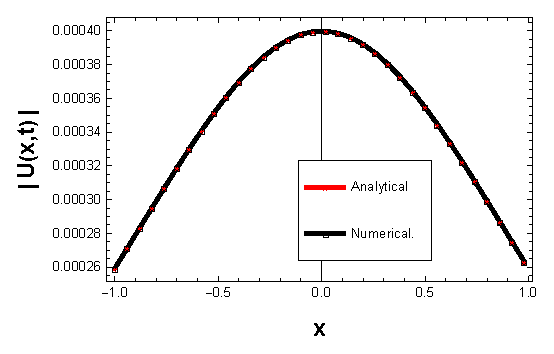
\includegraphics[width=11cm, height=6cm]{Figure1.eps}
 \caption{Analytical solutions and numerical results using collocation method with septic B-spline at $h = 0.02$ and $k = 0.00001$}
 \label{f.2}
\end{figure}

\textbf{case 2:} Let use step sizes h = 0.02, k = 0.0001. We then apply collocation with septic B-splines to find approximate solutions for this example.

\begin{table}[H]
 \centering
 \small
  \caption{Analytical solutions and numerical results using collocation method with septic B-spline at $k = 0.0001$ and $h = 0.02$}
  \label{T.4}
  \renewcommand{\arraystretch}{1.1}
  \begin{tabular}{|c|c|c|c|}
   \hline
   \textbf{$x_{i}$} & \textbf{Approx. solution} & \textbf{Analytical solution} & \textbf{Absolute error} \\ \hline
   -1.0 & 0.0259217 & 0.0259218 & $6.91335\times10^{-8}$ \\ \hline
   -0.8 & 0.0299075 & 0.0299074 & $6.58942\times10^{-8}$ \\ \hline
   -0.6 & 0.0337412 & 0.0337412 & $9.99861\times10^{-11}$ \\ \hline
   -0.4 & 0.0369992 & 0.0369992 & $1.36453\times10^{-13}$ \\ \hline
   -0.2 & 0.0392119 & 0.0392119 & $1.12479\times10^{-14}$ \\ \hline
   0.0 & 0.0399987 & 0.0399987 & $1.38431\times10^{-14}$ \\ \hline
   0.2 & 0.0392119 & 0.0392119 & $1.22749\times10^{-14}$ \\ \hline
   0.4 & 0.0369992 & 0.0369992 & $1.34205\times10^{-13}$ \\ \hline
   0.6 & 0.0337412 & 0.0337412 & $9.99851\times10^{-11}$ \\ \hline
   0.8 & 0.0299075 & 0.0299074 & $6.58942\times10^{-8}$ \\ \hline
   1.0 & 0.0259217 & 0.0259218 & $6.91335\times10^{-8}$ \\ \hline
  \end{tabular}
 \end{table}

\begin{figure}[H]
 \centering
 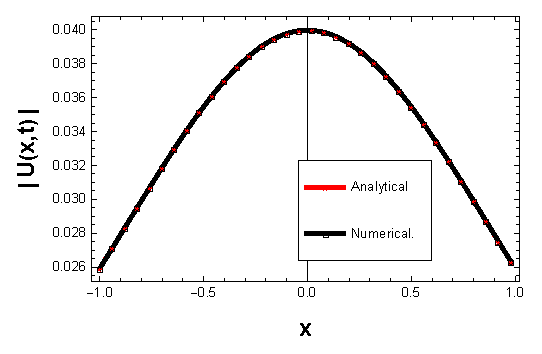
\includegraphics[width=11cm, height=6.5cm]{Figure2.eps}
 \caption{Analytical solutions and numerical results using collocation method with septic B-spline at $k = 0.0001$ and $h = 0.02$}
 \label{f.4}
\end{figure}

\begin{table}[H]
 \centering
 \small
 \caption{Comparison of absolute errors for Septic scheme and \cite{35} at $k = 0.00001$}
 \label{T.01}
 \renewcommand{\arraystretch}{1.1}
 \begin{tabular}{|c|c|c|}
  \hline
  \textbf{$x_{i}$} & \textbf{Present Septic Scheme} & \textbf{Quintic Scheme \cite{35}} \\ \hline 
  -1.0 & $6.84569\times10^{-14}$ & $4.07165 \times 10^{-14}$ \\ \hline
  -0.8 & $8.72697\times10^{-14}$ & $8.09859 \times 10^{-14}$ \\ \hline
  -0.6 & $1.68485\times10^{-16}$ & $2.56743 \times 10^{-14}$ \\ \hline
  -0.4 & $2.1684\times10^{-19}$ & $1.70627 \times 10^{-13}$ \\ \hline
  -0.2 & $5.42101\times10^{-19}$ & $1.07223 \times 10^{-13}$ \\ \hline
  0.0  & $5.96311\times10^{-19}$ & $1.27641 \times 10^{-13}$ \\ \hline
  0.2  & $4.87891\times10^{-19}$ & $1.47017 \times 10^{-13}$ \\ \hline
  0.4  & $2.71051\times10^{-19}$ & $1.26219 \times 10^{-13}$ \\ \hline
  0.6  & $1.69136\times10^{-16}$ & $2.60316 \times 10^{-13}$ \\ \hline
  0.8  & $8.72703\times10^{-14}$ & $3.04785 \times 10^{-14}$ \\ \hline
  1.0  & $6.84569\times10^{-14}$ & $9.40076 \times 10^{-14}$ \\ \hline
 \end{tabular}
\end{table}

\begin{table}[H]
 \centering
 \small
  \caption{Comparison of absolute errors for Septic scheme and \cite{35} at $k = 0.0001$}
  \label{T.02}
  \renewcommand{\arraystretch}{1.1}
  \begin{tabular}{|c|c|c|}
   \hline
   \textbf{$x_{i}$} & \textbf{Present Septic Scheme} & \textbf{Quintic Scheme \cite{35}} \\ \hline
   -1.0 & $6.91335\times10^{-8}$ & $6.91416\times10^{-8}$ \\ \hline
   -0.8 & $6.58942\times10^{-8}$ & $5.26461\times10^{-9}$ \\ \hline
   -0.6 & $9.99861\times10^{-11}$ & $7.11724\times10^{-12}$ \\ \hline
   -0.4 & $1.36453\times10^{-13}$ & $1.25044\times10^{-11}$ \\ \hline
   -0.2 & $1.12479\times10^{-14}$ & $1.62707\times10^{-11}$ \\ \hline
   0.0 & $1.38431\times10^{-14}$ & $2.023\times10^{-11}$ \\ \hline
   0.2 & $1.22749\times10^{-14}$ & $1.94917\times10^{-11}$ \\ \hline
   0.4 & $1.34205\times10^{-13}$ & $1.67006\times10^{-11}$ \\ \hline
   0.6 & $9.99851\times10^{-11}$ & $1.78017\times10^{-11}$ \\ \hline
   0.8 & $6.58942\times10^{-8}$ & $5.23189\times10^{-9}$ \\ \hline
   1.0 & $6.91335\times10^{-8}$ & $6.91253\times10^{-8}$ \\ \hline
  \end{tabular}
 \end{table}

Tables \ref{T.2} and \ref{T.4}, together with Figures \ref{f.2} and \ref{f.4}, compare the numerical outcomes obtained using the septic B-spline approach with the analytical solution (\ref{p1.01}) of Eq.(\ref{p1.1}), which corresponds to the sine-Gordon equation, under two different cases. The close agreement between the numerical and analytical results confirms the validity of the analytical solution and demonstrates the effectiveness of the numerical scheme. For the prescribed parameter values, the solutions of Eq.(\ref{p1.1}) exhibit characteristic behaviors that are clearly illustrated in Tables \ref{T.2} and \ref{T.4} and Figures \ref{f.2} and \ref{f.4}. Moreover, these comparisons emphasize the accuracy and reliability of both the analytical and numerical approaches and demonstrate the efficiency of the combined analytical--numerical framework in analyzing the sine-Gordon equation.

Tables \ref{T.01} and \ref{T.02} report the absolute errors obtained by the numerical approach proposed in this study and those produced by the method presented in \cite{35}. The results indicate that the septic B-spline approach consistently yields smaller absolute errors than the quintic B-spline, demonstrating higher accuracy.

\textbf{Test problem 2:}

In this example, we solve Eq \ref{p1.1} by using:

Initial conditions.
\begin{eqnarray*}
 u(x,0) &=&\sin(\pi x), \\
 u_{t}(x,0) &=&0.
\end{eqnarray*}
Boundary conditions
\begin{equation*}
 u(0,t)=u(1,t)=0,\ \ \ \forall\ t>0
\end{equation*}
Analytical solution is: \cite{27}
\begin{equation}\label{p1.02}
 u(x,t)=\frac{1}{2}(\sin \pi (x+t)+\sin \pi (x-t))
\end{equation}

\textbf{case 1:} For the domain, $0\leq x\leq 1$, test Problem 2 is solved using the septic B-spline approach. The computations use the parameters $ k = 0.00001 $ and a spatial step size of $ h = \frac{1}{300} $

\begin{table}[H]
 \centering
 \small
  \caption{Analytical solutions and numerical results using collocation method with septic B-spline at $h =\frac{1}{300}$ and $k = 0.00001$}
  \label{Table 02}
  \renewcommand{\arraystretch}{1.1}
  \begin{tabular}{|c|c|c|c|}
   \hline
   \textbf{$x_i$} & \textbf{Approx. solution} & \textbf{Analytical solution} & \textbf{Absolute error} \\ 
   \hline
   0.    & 0.0000314159 & 0.    & 0.0000314159 \\ \hline
   0.1   & 0.309017     & 0.309017     & \(9.12226 \times 10^{-9}\) \\ \hline
   0.2   & 0.587785     & 0.587785     & \(1.66356 \times 10^{-8}\) \\ \hline
   0.3   & 0.809017     & 0.809017     & \(2.17083 \times 10^{-8}\) \\ \hline
   0.4   & 0.951056     & 0.951056     & \(2.44209 \times 10^{-8}\) \\ \hline
   0.5   & 0.99999966           & 0.99999969           & \(2.52441 \times 10^{-8}\) \\ \hline
   0.6   & 0.951056     & 0.951056     & \(2.44209 \times 10^{-8}\) \\ \hline
   0.7   & 0.809017     & 0.809017     & \(2.17083 \times 10^{-8}\) \\ \hline
   0.8   & 0.587785     & 0.587785     & \(1.66356 \times 10^{-8}\) \\ \hline
   0.9   & 0.309017     & 0.309017     & \(9.12367 \times 10^{-9}\) \\ \hline
   1.    & \(2.4941 \times 10^{-15}\) & 0 & \(2.4941 \times 10^{-15}\) \\ \hline
  \end{tabular}
 \end{table}

\begin{figure}[H]
 \centering
 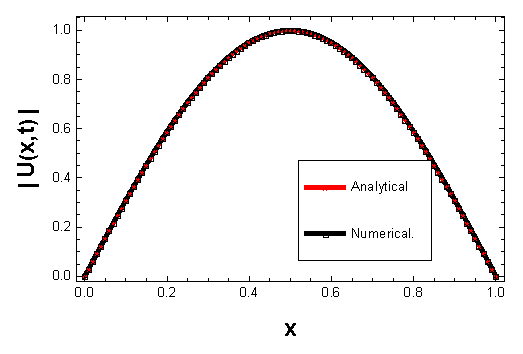
\includegraphics[width=10cm, height=6cm]{Figure3.eps}
 \caption{Analytical solutions and numerical results using collocation method with septic B-spline at $h =\frac{1}{300}$ and $k = 0.00001$}
 \label{f.5}
\end{figure}

\textbf{case 2:} For the domain, $-1\leq x\leq 1$, test Problem 2 is solved using the septic B-spline approach. The computations use the parameters $ k = 0.001 $ and a spatial step size of $ h = 0.02 $

\begin{table}[H]
 \centering
 \small
  \caption{Analytical solutions and numerical results using collocation method with septic B-spline at $h = 0.02$ and $k = 0.001$}
  \label{Table 002}
  \renewcommand{\arraystretch}{1.1}
  \begin{tabular}{|c|c|c|c|}
   \hline
   \textbf{$x_i$} & \textbf{Approx. solution} & \textbf{Analytical solution} & \textbf{Absolute error} \\ 
   \hline
  -1.   & 0.00785392     & \(1.21431 \times 10^{16}\) & 0.00785392 \\ \hline
  -0.8  & 0.587458       & 0.587495     & 0.0000368989 \\ \hline
  -0.6  & 0.950551       & 0.950587     & 0.0000366415 \\ \hline
  -0.4  & 0.950551       & 0.950587     & 0.0000366272 \\ \hline
  -0.2  & 0.58747        & 0.587495     & 0.0000249487 \\ \hline
  0.    & \(1.69309 \times 10^{-15}\) & 0.    & \(1.69309 \times 10^{-15}\) \\ \hline
  0.2   & 0.58747        & 0.587495     & 0.0000249487 \\ \hline
  0.4   & 0.950551       & 0.950587     & 0.0000366272 \\ \hline
  0.6   & 0.950551       & 0.950587     & 0.0000366272 \\ \hline
  0.8   & 0.58747        & 0.587495     & 0.0000249518 \\ \hline
  1.    & \(1.38084 \times 10^{-15}\) & \(1.21431 \times 10^{-16}\) & \(1.25941 \times 10^{-15}\) \\  \hline
  \end{tabular}
 \end{table}

\begin{figure}[H]
 \centering
 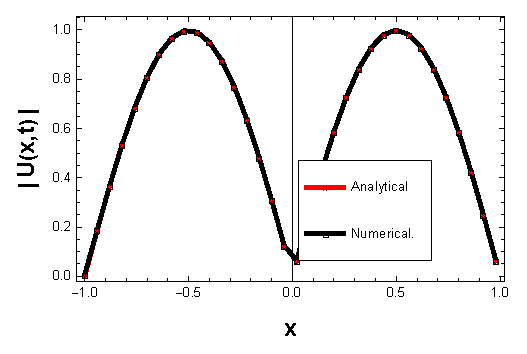
\includegraphics[width=10cm, height=5cm]{Figure4.eps}
 \caption{Analytical solutions and numerical results using collocation method with septic B-spline at $h = 0.02$ and $k = 0.001$}
 \label{f.6}
\end{figure}

\begin{table}[H]
 \centering
 \small
 \caption{Comparison of absolute errors for Septic scheme and \cite{24} at $k = 0.00001$}
 \label{Table 0001}
 \renewcommand{\arraystretch}{1.1}
 \begin{tabular}{|c|c|c|}
  \hline
  \textbf{$x_{i}$} & \textbf{Present Septic Scheme} & \textbf{finite differences \cite{24}} \\ \hline 
  0.0   & 0.0000314159 & 0 \\ \hline
  0.1   & \(9.12226 \times 10^{-9}\) & \(1.22915 \times 10^{-7}\) \\ \hline
  0.2   & \(1.66356 \times 10^{-8}\) & \(2.2194 \times 10^{-7}\) \\ \hline
  0.3   & \(2.17083 \times 10^{-8}\) & \(2.85862 \times 10^{-7}\) \\ \hline
  0.4   & \(2.44209 \times 10^{-8}\) & \(3.17923 \times 10^{-7}\) \\ \hline
  0.5   & \(2.52441 \times 10^{-8}\) & \(3.27131 \times 10^{-7}\) \\ \hline
  0.6   & \(2.44209 \times 10^{-8}\) & \(3.17923 \times 10^{-7}\) \\ \hline
  0.7   & \(2.17083 \times 10^{-8}\) & \(2.85862 \times 10^{-7}\) \\ \hline
  0.8   & \(1.66356 \times 10^{-8}\) & \(2.2194 \times 10^{-7}\) \\ \hline
  0.9   & \(9.12367 \times 10^{-9}\) & \(1.22915 \times 10^{-7}\) \\ \hline
  1.0   & \(2.4941 \times 10^{-15}\) & 0 \\ \hline
 \end{tabular}
\end{table}

\begin{table}[H]
 \centering
 \small
 \caption{Comparison of absolute errors for Septic scheme and \cite{38} at $k = 0.001$}
 \label{Table 001}
 \renewcommand{\arraystretch}{1.1}
 \begin{tabular}{|c|c|c|}
  \hline
  \textbf{$x_{i}$} & \textbf{Present Septic Scheme} & \textbf{Quadratic Scheme \cite{38}} \\ \hline 
 -1.0   & 0.00785392 & 0.000512099 \\ \hline
 -0.8   & 0.0000368989 & 0.00161248  \\ \hline
 -0.6   & 0.0000366415 & 0.00230875  \\ \hline
 -0.4   & 0.0000366272 & 0.00216485  \\ \hline
 -0.2   & 0.0000249487 & 0.00120944  \\ \hline
 0.0    & \(1.69309 \times 10^{-15}\) & 0.00025929  \\ \hline
 0.2    & 0.0000249487 & 0.00161247  \\ \hline
 0.4    & 0.0000366272 & 0.00230875 \\ \hline
 0.6    & 0.0000366272 & 0.00216485 \\ \hline
 0.8    & 0.0000249518 & 0.00120945 \\ \hline
 1.0    & \(1.25941 \times 10^{-15}\) & \(6.48074 \times 10^{-6}\)  \\ \hline
 \end{tabular}
\end{table}

Tables \ref{Table 02} and \ref{Table 002}, together with Figures \ref{f.5} and \ref{f.6}, compare the numerical outcomes obtained using the septic B-spline approach with the analytical solution (\ref{p1.02}) of Eq.(\ref{p1.1}), which corresponds to the sine-Gordon equation, under two different cases. The close agreement between the numerical and analytical results confirms the validity of the analytical solution and demonstrates the effectiveness of the numerical scheme. For the prescribed parameter values, the solutions of Eq.(\ref{p1.1}) exhibit characteristic behaviors that are clearly illustrated in Tables \ref{Table 02} and \ref{Table 002} and Figures \ref{f.5} and \ref{f.6}. Moreover, these comparisons emphasize the accuracy and reliability of both the analytical and numerical approaches and demonstrate the efficiency of the combined analytical--numerical framework in analyzing the sine-Gordon equation.

Tables \ref{Table 0001} and \ref{Table 001} report the absolute errors obtained by the numerical approach proposed in this study and those produced by the methods presented in \cite{24,38}. The results indicate that the septic B-spline approach consistently yields smaller absolute errors than the other approaches, demonstrating higher accuracy. Notably, the collocation method with septic B-spline yields errors approximately one order of magnitude lower than the finite difference method \cite{24}, demonstrating the benefits of employing higher-order splines.

\textbf{Test problem 3:}

In this example, we solve Eq \ref{p1.1} by using:

Initial conditions.
\begin{eqnarray*}
 u(x,0) &=&f(x), \\
 u_{t}(x,0) &=&g(x),
\end{eqnarray*}
Boundary conditions
\begin{equation*}
 u(0,t)=u(1,t)=0,\ \ \ \forall\ t>0
\end{equation*}
Analytical solution is: \cite{39}
\begin{equation}\label{p1.002}
 u(x,t)=4 \tan^{-1}(e^{\gamma(x-c t)})
\end{equation}

\textbf{case 1:} For the domain, $0\leq x\leq 1$, test Problem 3 is solved using the collocation method with septic B-spline approach. The computations use the parameters $c = 0.5$, $\gamma= \frac{1}{\sqrt{1-c^2}},$ $ k = 0.00001 $ and a spatial step size of $ h = 0.01 $

\begin{table}[H]
 \centering
 \small
  \caption{Analytical solutions and numerical results using collocation method with septic B-spline at $h =0.01$ and $k = 0.00001$}
  \label{Table 0002}
  \renewcommand{\arraystretch}{1.1}
  \begin{tabular}{|c|c|c|c|}
   \hline
   \textbf{$x_i$} & \textbf{Approx. solution} & \textbf{Analytical solution} & \textbf{Absolute error} \\ 
   \hline
   0.    & 3.14147718353576  & 3.1414771835360193    & \(2.59348 \times 10^{-13}\) \\ \hline
   0.1   & 3.37190656020845     & 3.3719065602084415     & \(1.5099 \times 10^{-14}\) \\ \hline
   0.2   &  3.59930871578175     & 3.599308715781757     & \(4.44089 \times 10^{-16}\) \\ \hline
   0.3   & 3.82084942668103     & 3.820849426681035     & \(4.44089 \times 10^{-16}\) \\ \hline
   0.4   & 4.03405410046914     & 4.034054100469141     & \(8.88178 \times 10^{-16}\) \\ \hline
   0.5   & 4.23692181534061           & 4.236921815340607         & \(4.44089 \times 10^{-15}\) \\ \hline
   0.6   & 4.42797945208822     & 4.427979452088221    & \(8.88178 \times 10^{-16}\) \\ \hline
   0.7   & 4.60627972335831     &  4.606279723358314    & \(8.88178 \times 10^{-16}\) \\ \hline
   0.8   &  4.77135576593184     & 4.7713557659318475     & \(7.10543 \times 10^{-15}\) \\ \hline
   0.9   & 4.92314861658900     & 4.92314861658908   & \(7.54952 \times 10^{-14}\) \\ \hline
   1.    & 5.06192307734576 & 5.061923077345729 & \(3.28626 \times 10^{-14}\) \\ \hline
  \end{tabular}
 \end{table}

\begin{figure}[H]
 \centering
 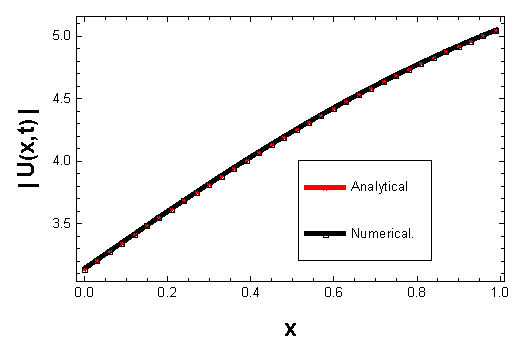
\includegraphics[width=11cm, height=6.5cm]{Figure5.eps}
 \caption{Analytical solutions and numerical results using collocation method with septic B-spline at $h =0.01$ and $k = 0.00001$}
 \label{f.05}
\end{figure}

\begin{figure}[H]
 \centering
 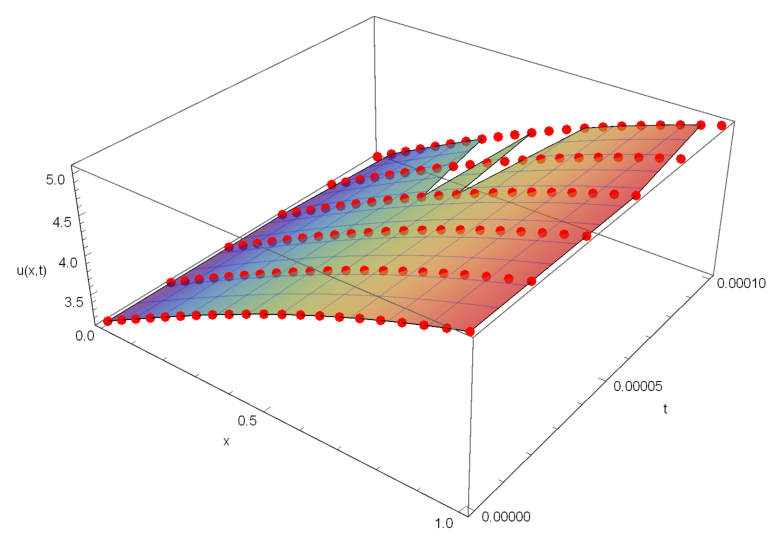
\includegraphics[width=11cm, height=6.5cm]{Figure6.eps}
 \caption{3D plot of the numerical and analytical solutions for Test Problem 3}
 \label{f.005}
\end{figure}

To provide a visual assessment of the method's accuracy, Figure \ref{f.005} displays a 3D surface plot comparing the numerical and analytical solutions. The numerical solution (blue surface) obtained using the collocation method with septic B-spline shows excellent agreement with the analytical solution (red points), confirming the reliability and precision of the proposed approach for solving the sine-Gordon equation.

\section{Conclusion}
In this study, analytical and numerical solutions to selected test problems were obtained using the proposed approach. The absolute error analysis demonstrates that the method provides accurate and reliable approximations for the sine-Gordon equation when employing the collocation method with septic B-splines. Furthermore, the stability analysis confirms that the proposed scheme is conditionally stable, highlighting its effectiveness in solving this equation. Despite these advantages, the proposed approach has certain drawbacks. The conditional nature of the stability imposes restrictions on the time step size, particularly when using fine spatial grids. Moreover, the computational implementation is more demanding compared to collocation method with cubic or quintic B-spline, as the collocation method with septic B-spline formulation requires solving matrices with a larger bandwidth. Future investigations could focus on generalizing the scheme to higher-dimensional problems, incorporating adaptive refinement techniques for problems exhibiting sharp gradients, and testing the method on other nonlinear evolution equations, such as the Klein-Gordon equation.

\begin{thebibliography}{99}

\bibitem[1]{1} J. K. Perring, T. H. R. Skyrme, A model unified field equation, Nuclear Physics, 31, 550--555, (1962). \href{https://doi.org/10.1016/0029-5582(62)90774-5}{https://doi.org/10.1016/0029-5582(62)90774-5}

\bibitem[2]{2} G. Ben-Yu, P. J. Pascual, M. J. Rodriguez, and L. Vazquez, Numerical solution of the sine-Gordon equation, Applied Mathematics and Computation, 18(1), 1--14, (1986).

\bibitem[3]{3} A. G. Bratsos, E. H. Twizell, The solution of the sine Gordon equation using the method of lines, International Journal of Computer Mathematics, 61(3-4), 271--292, (1996).

\bibitem[4]{4} A. Mohebbi, M. Dehghan, High-order solution of one dimensional sine-Gordon equation using compact finite difference and DIRKN methods, Mathematical and Computer Modelling, 51(5-6), 537--549, (2010).

\bibitem[5]{5} Sc. Evry, A theory of the role of magnetic activity during star formation, Annales d'Astrophysique, 25, (1962).

\bibitem[6]{6} A. M. A. El-Sayed, On the fractional differential equations, Appl. Math. Comp, 49(2-3), (1992). \href{https://doi.org/10.1016/0096-3003(92)90024-U}{https://doi.org/10.1016/0096-3003(92)90024-U}

\bibitem[7]{7} Ketabchi S., Moosaei H., Fallahi S., Optimal error correction of the absolute value equation using a genetic algorithm, Mathematical and Computer Modelling, 57(9-10), 2339--2342, (2013).

\bibitem[8]{8} T. D. Taylor, E. Ndefo, B. S. Masson, A study of numerical methods for solving viscous and inviscid flow problems, Journal of Computational Physics, 9(1), 99--119, (1972).

\bibitem[9]{9} A. B. Shamardan, Y. M. Essa, Multi-level adaptive solutions to initial-value problems, Korean Journal of Computational and Applied Mathematics, 7(1), 215--222, (2000).

\bibitem[10]{10} Ch. Ian, Product approximation for non-linear problems in the finite element method, IMA Journal of Numerical Analysis, 1(3), 253--266, (1981). \href{https://doi.org/10.1093/imanum/1.3.253}{https://doi.org/10.1093/imanum/1.3.253}

\bibitem[11]{11} A. A. Soliman, Exact travelling wave solution of nonlinear variants of the RLW and the PHI-four equations, Physics Letters A, 368(5), 383--390, (2007). \href{https://doi.org/10.1016/j.physleta.2007.04.038}{https://doi.org/10.1016/j.physleta.2007.04.038}

\bibitem[12]{12} A. A. Soliman, Exact solutions of KdV-Burgers' equation by Exp-function method, Chaos, Solitons \& Fractals, 41(2), 1034--1039, (2009).

\bibitem[13]{13} A. A. Soliman, M. A. Abdou, ``Exact travelling wave solutions of nonlinear partial differential equations'', Chaos, Solitons \& Fractals, 32, 808--815, (2007).

\bibitem[14]{14} A. A. Soliman, M. A. Abdou, ``The Decomposition Method for Solving the Coupled Modified KdV Equations'', Mathematical and Computer Modelling, 47(9-10), 1035--1041, (2008). \href{https://doi.org/10.1016/j.mcm.2007.05.012}{https://doi.org/10.1016/j.mcm.2007.05.012}

\bibitem[15]{15} A. A. Soliman, On the solution of two-dimensional coupled Burgers' equations by variational iteration method, Chaos, Solitons \& Fractals, 40(3), 1146--1155, (2009). \href{https://doi.org/10.1016/j.chaos.2007.08.069}{https://doi.org/10.1016/j.chaos.2007.08.069}

\bibitem[16]{16} A. A. Soliman, A. H. A. Ali and K. R. Raslan, Numerical Solution for the KdV Equation Based on Similarity Reductions, Applied Mathematical Modelling, 33(2), 1107--1115, (2009).

\bibitem[17]{17} A. A. Soliman, Numerical Simulation of the FitzHugh-Nagumo equations, Abstract and Applied Analysis, Vol. 2012, Pages 13, (2012).

\bibitem[18]{18} A. A. Soliman, A Galerkin solution for Burgers' equation using cubic B-spline finite elements, Abstract and Applied Analysis, Vol. 2012, Article ID 527467, (2012). \href{https://doi.org/10.1155/2012/527467}{https://doi.org/10.1155/2012/527467}

\bibitem[19]{19} A. A. Soliman, K. R. Raslan, A. M. Abdallah, On Some Modified Methods on Fractional Delay and Nonlinear Integro-Differential Equation, Sound \& Vibration, 55(4):263--279, (2021). \href{https://doi.org/10.32604/sv.2021.015014}{https://doi.org/10.32604/sv.2021.015014}

\bibitem[20]{20} A. A. Soliman and K. R. Raslan, ``Collocation Method using quadratic B-Spline for RLW Equation'', International Journal of Computer Mathematics, Vol. 78, P. 399--412, (2001). \href{https://doi.org/10.1080/00207160108805119}{https://doi.org/10.1080/00207160108805119}

\bibitem[21]{21} A. A. Soliman, ``Collocation Solution of the Korteweg-De Vries Equation using Septic Splines'', International Journal of Computer Mathematics, Vol. 81, 325--331, (2004). \href{https://doi.org/10.1080/00207160410001660817}{https://doi.org/10.1080/00207160410001660817}

\bibitem[22]{22} A. A. Soliman, M. H. Hussien, ``Collocation Solution for RLW Equation with Septic Spline'', Applied Mathematics and Computation, 161, 623--636, (2005).

\bibitem[23]{23} A. A. Soliman, Collocation Method using Quartic B-Splines for Solving the Modified RLW Equation, Indian Journal of Science and Technology, 10(31), August, (2017).

\bibitem[24]{24} K. R. Raslan, A. A. Soliman, Kh. Ali, M. Gaber, S. Almhdy, Numerical Solution for the Sin-Gordon Equation Using Finite Difference Method and the Non-stander Finite Difference Method, Appl. Math. Inf. Sci., 17(2), 1--8, (2023).

\bibitem[25]{25} A. A. Soliman, Manar M. Dahshan, Ahmed S. Elgazzar, A finite difference scheme for the two-dimensional sine-Gordon equation, Delta Journal of Science, Vol. 50(1)--pp. 45--53, (2025).

\bibitem[26]{26} A. A. Soliman, K. R. Raslan, Kh. Ali, A. S. Awad, Numerical Simulation for the Two-Dimensional Partial Differential Equations, Delta Journal of Science, Vol. 51(1)--pp. 141--158, (2025).

\bibitem[27]{27} A. A. Soliman, Finite Element Method for Solving the Generalized RLW Equation, ICCFD 2014 : XII International Conference on Computational Fluid Dynamics, Amsterdam, The Netherlands, (2014).

\bibitem[28]{28} A. A. Soliman, Collocation method using quartic B-splines for solving the Modified RLW Equation, 4th International Conference on Computer Science \& Computational Mathematics, May 7-8, 2015, Langkawi, Malaysia.

\bibitem[29]{29} K. Ramaz, J. Leon, Bistability in the sine-Gordon equation: The ideal switch, Physical Review E, 71(5), (2005). \href{https://doi.org/10.1103/PhysRevE.71.056620}{https://doi.org/10.1103/PhysRevE.71.056620}

\bibitem[30]{30} K. R. Raslan, Numerical methods for partial differential equations, PhD thesis, Azhar University, Cairo, (1999).

\bibitem[31]{31} S. Granville, The numerical solution of ordinary and partial differential equations, John Wiley \& Sons, 75, (2005).

\bibitem[32]{32} Johnson S., P. Suarez, and A. Biswas, New exact solutions for the sine-Gordon equation in 2+1 dimensions, Computational Mathematics and Mathematical Physics, 52(1), 98--104, (2012). \href{https://doi.org/10.1134/S0965542512010058}{https://doi.org/10.1134/S0965542512010058}

\bibitem[33]{33} K. R. Raslan, T. S. El-Danaf, K. K. Ali, Application of septic B-spline collocation method for solving the coupled-BBM system, Appl Comput Math, 5(5), 2--7, (2016).

\bibitem[34]{34} I. Dag, D. Irk, and B. Saka, Numerical Solution of the Burgers equation using cubic B-splines, Applied Mathematics and Computation, 163(1), 199--211, (2005).

\bibitem[35]{35} A. A. Soliman, K. R. Raslan, A. S. Awad, Numerical solutions for the Sine-Gordon equation based on the Quintic B-Spline approach, Arish Journal of Science, Accepted, (2025).

\bibitem[36]{36} M. T. Darvishi, F. Khani, S. Hamedi-Nezhad, Sang-Wan Ryu, New modification of the HPM for numerical solutions of the sine-Gordon and coupled sine-Gordon equations, International Journal of Computer Mathematics, Vol. 87, no. 4, 908--919, (2010). \href{https://doi.org/10.1080/00207160802247596}{https://doi.org/10.1080/00207160802247596}

\bibitem[37]{37} Y. Salehi, M. T. Darvishi, W. E. Schiesser, Numerical solution of space fractional diffusion equation by the method of lines and splines, Applied Mathematics and Computation, 336, 465--480, (2018). \href{https://doi.org/10.1016/j.amc.2018.04.053}{https://doi.org/10.1016/j.amc.2018.04.053}

\bibitem[38]{38} Soma R. Almhdy, Some numerical solutions for some equations related to wave equation, MSc thesis, Arish University, Al-Arish, (2023).

\bibitem[39]{39} J. Rashidinia and R. Mohammadi, Tension spline solution of nonlinear sine-Gordon equation, Numerical Algorithms, 56(1), 129--142, (2011). \href{https://doi.org/10.1007/s11075-010-9377-x}{https://doi.org/10.1007/s11075-010-9377-x}


\end{thebibliography}

\end{document}